\section{Experiment \& Result} \label{section:experiment_result}

In this section, first, we present our experiment result on Oxford 5K Building Dataset to prove that our BoW implementation can achieve good enough performance on standard benchmark. The experiment shows that our version of BoW achieves the mean average precision of 0.844 on Oxford 5K Building Dataset with nearly one second average time for each query. This dataset was constructed by Philbin et al. in 2007 \cite{2}. It consists of 5,062 images of resolution $1024 \times 768$ belongs to 11 different Oxford buildings. Images for each building are collected from Flickr by searching using text queries. In figure \ref{fig:oxbuilding}, some samples from the dataset are shown. Along with the dataset, there are also 55 queries along with their ground-truth, 5 for each landmark, as shown in figure \ref{fig:oxbuilding_query}. The ground truth of 55 queries are manually constructed. For each query, images are classified into 4 groups: (1) \textit{Good}: the building appears apparently, (2) \textit{OK}: more than 25\% of the building is present, (3) \textit{Bad}: the building is not shown up, and (4) \textit{Junk}: less than 25\% of the building is captured. The reason why the authors use this dataset is because of its popularity, it is used by many previous works in this field. Thus, we can easily compare our systems with those previous works.

Secondly, we also present and illustrate several typical scenarios of our automatic annotation system with the dataset consisting of our personal photos taken from Facebook. This dataset includes 6 different classes corresponding with 6 social events. Photos in each class share some particular attributes such as background, mascots, logos. As a result, whenever a photo is tagged, other photos in the same class can also be tagged similarly thanks to theses mutual attributes. The details of these 6 classes in the dataset are described below:

\begin{enumerate}

\item \#APCS\_Party: Photos taken at a party of my university. Photos in this class contain nearly the same group of people and have similar background and light conditions. Examples are given in Fig. \ref{fig:class_1}.
\item \#First\_time\_in\_Singapore: These photos are taken at the Merlion in Singapore. They all contain the merlion statue. Examples are given in Fig. \ref{fig:class_2}.
\item \#Hoi\_An\_with\_family: These photos are taken at Hoi An town in Vietnam with one of the authors' family. The people appearing in them and the background are their common attributes. Examples are given in Fig. \ref{fig:class_3}.
\item \#My\_favoriate\_competition: These are taken at multiple times I have taken part in the ACM-ICPC, a really famous collegiate programming competition. The mutual characteristic of these photos is the logo of the competition. Examples are given in Fig. \ref{fig:class_4}.
\item \#My\_first\_regional: These photos are taken at my ICPC regional contest in Phuket, Thailand. The photos all accommodate the mascot of the competition. Examples are given in Fig. \ref{fig:class_5}.
\item \#Odon\_Vallet: These photos are taken at the Odon Vallet scholarship ceremony. Their common features are the formal clothes (white T-shirts and dark trousers) and also the background. Examples are given in Fig. \ref{fig:class_6}.

\end{enumerate}

\begin{figure}
    \centering
	\subfloat{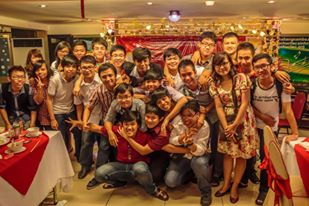
\includegraphics[width = 2in]{APCS_4.jpg}}
	\subfloat{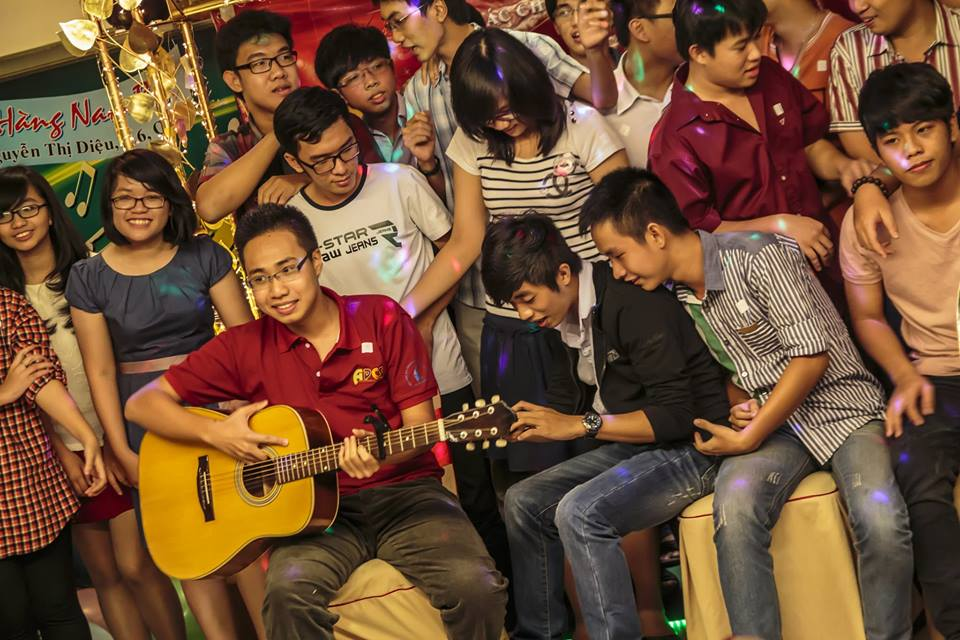
\includegraphics[width = 2in]{APCS_2.jpg}}
	\subfloat{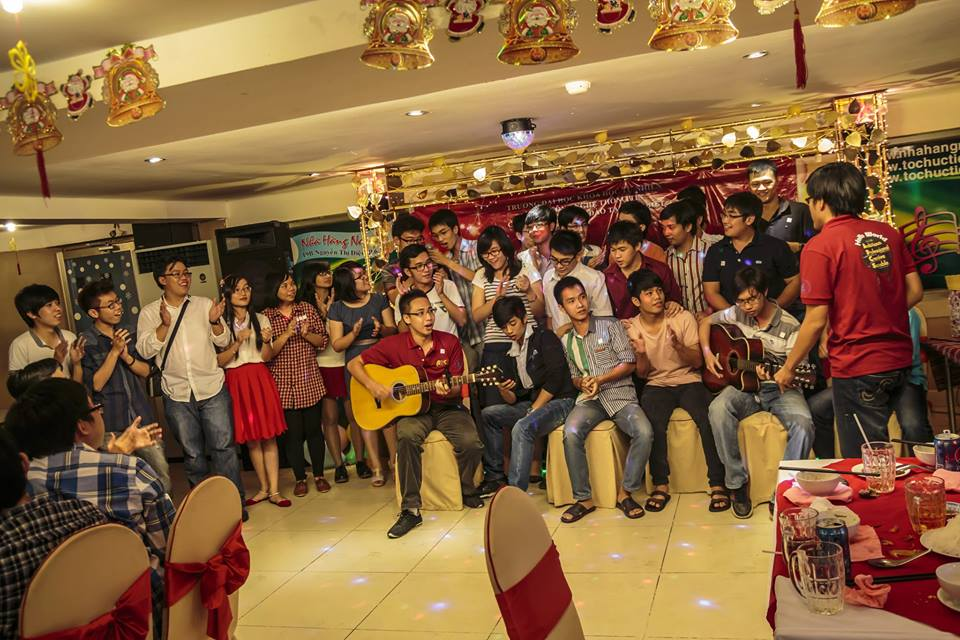
\includegraphics[width = 2in]{APCS_3.jpg}}
    \caption{Class 1, \#APCS\_Party}
    \label{fig:class_1}
\end{figure}

\begin{figure}
    \centering
	\subfloat{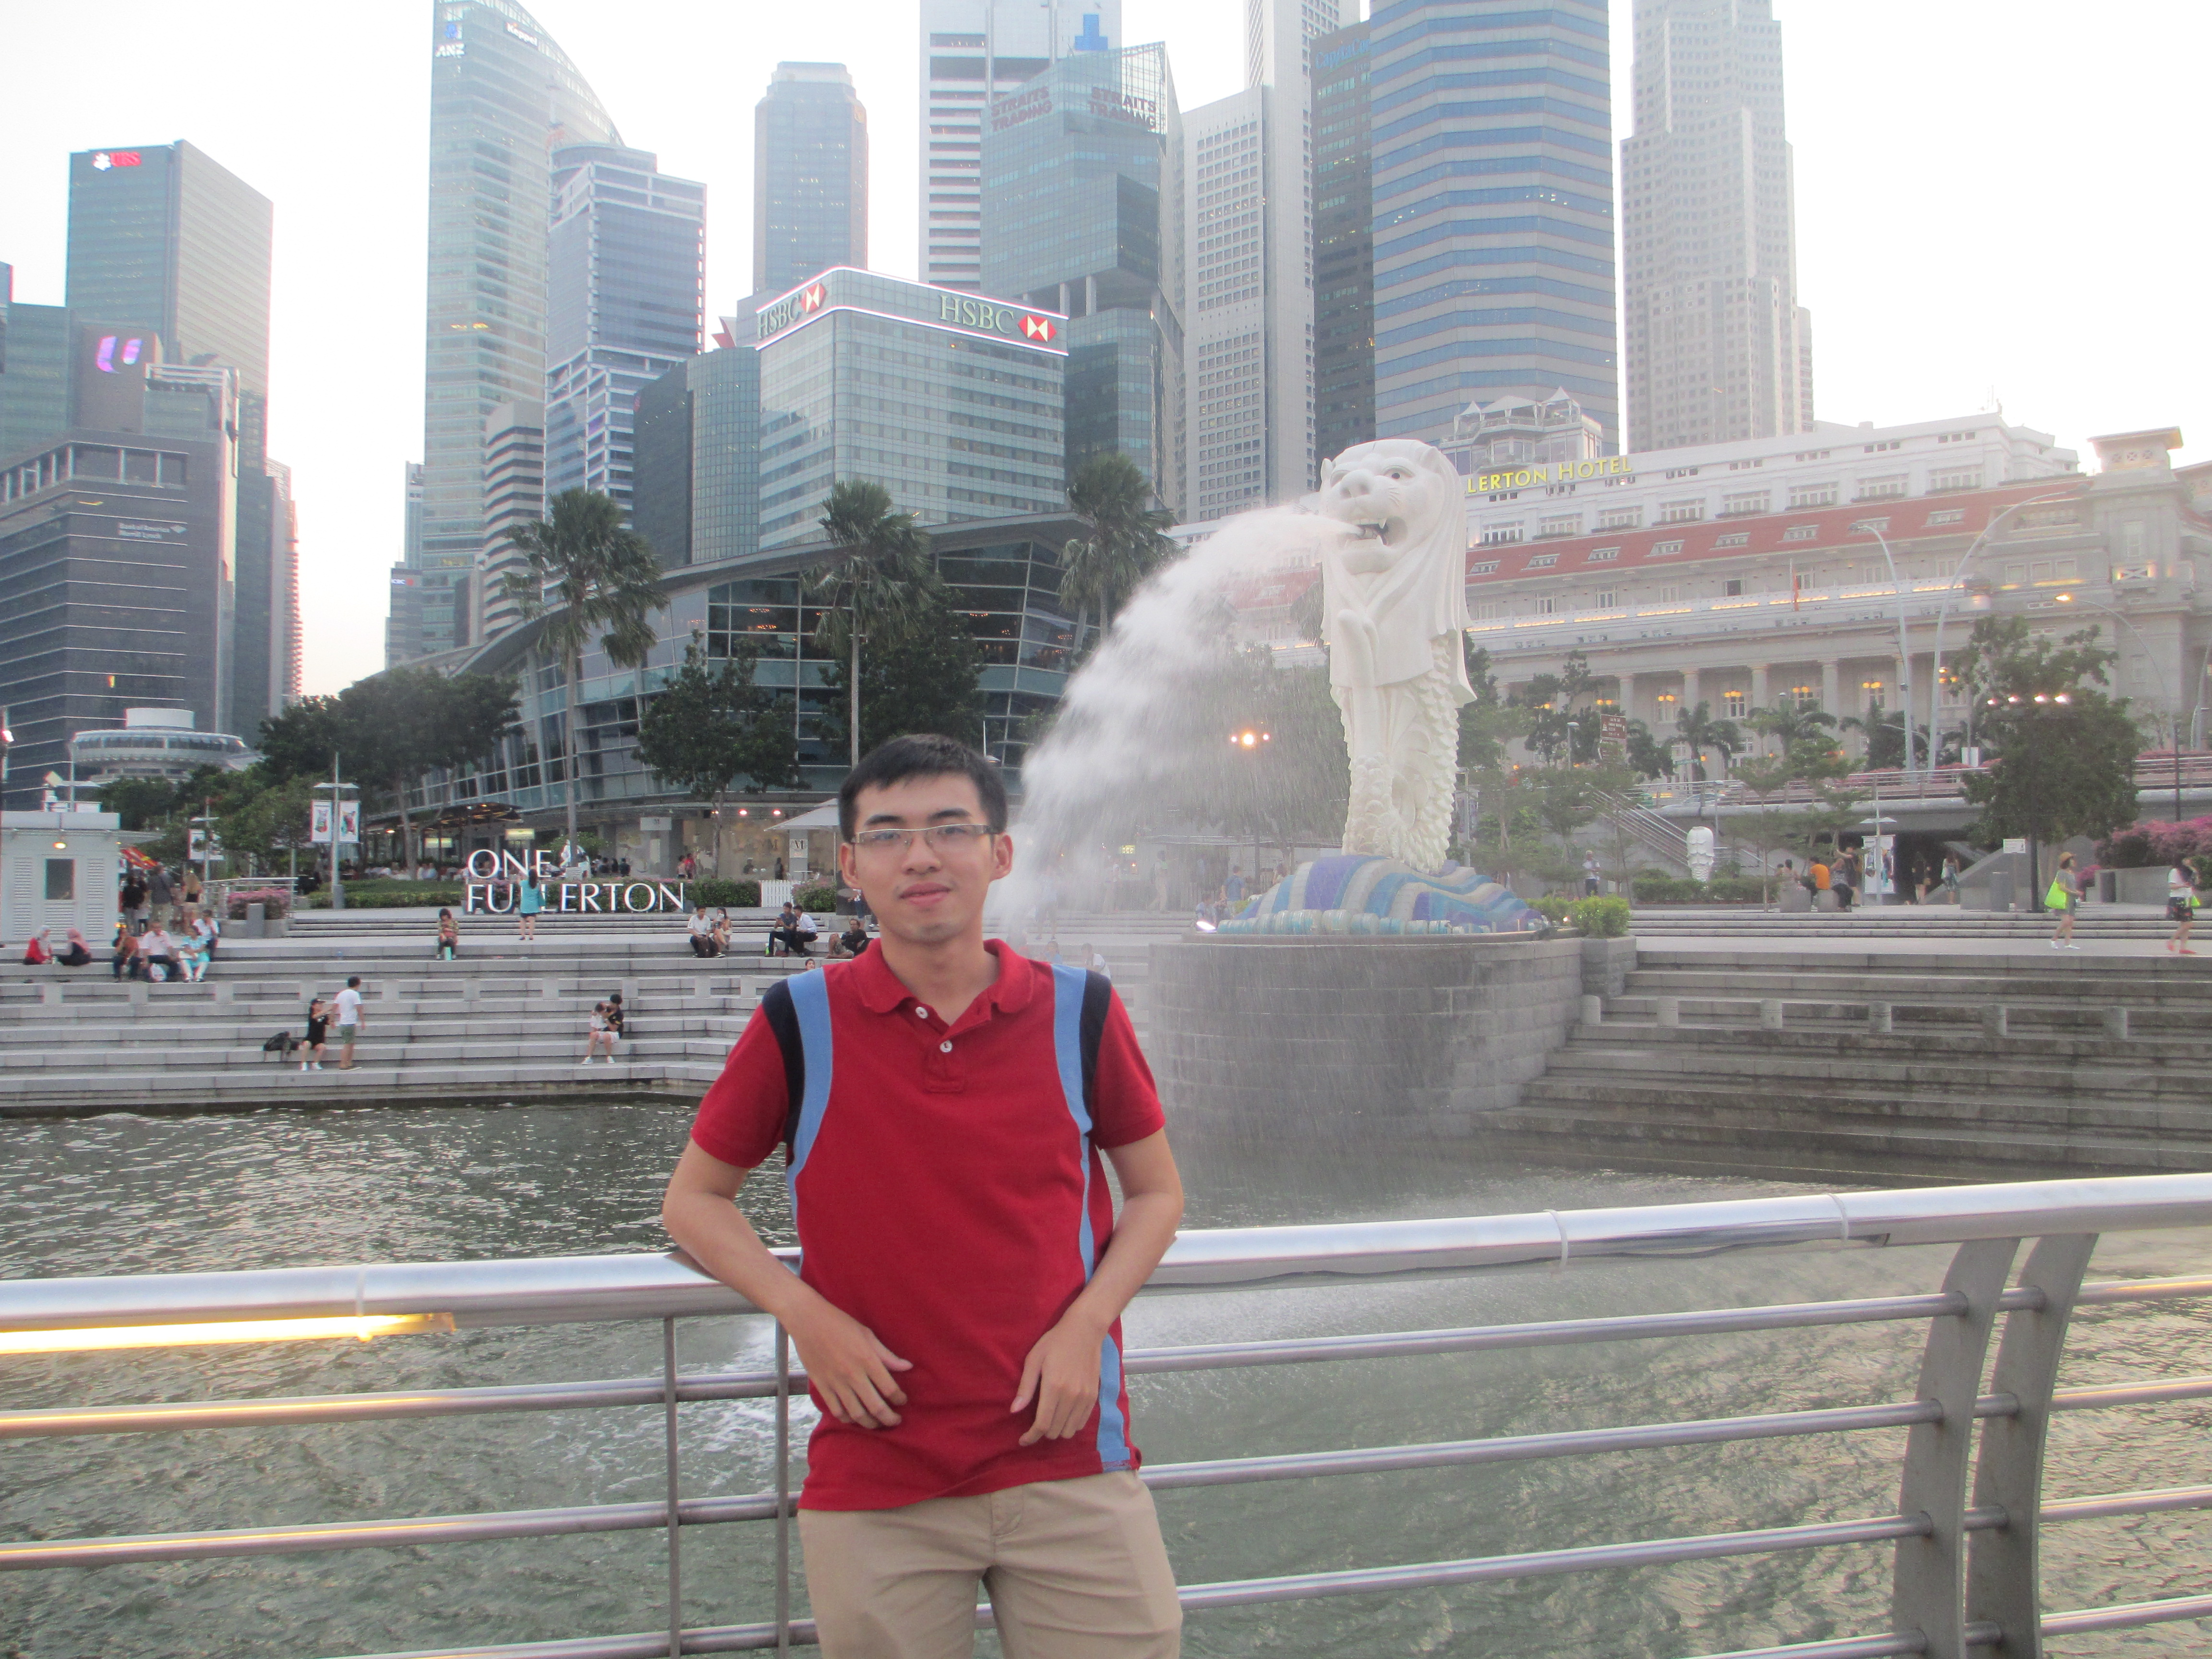
\includegraphics[width = 2in]{singapore_2.jpg}}
	\subfloat{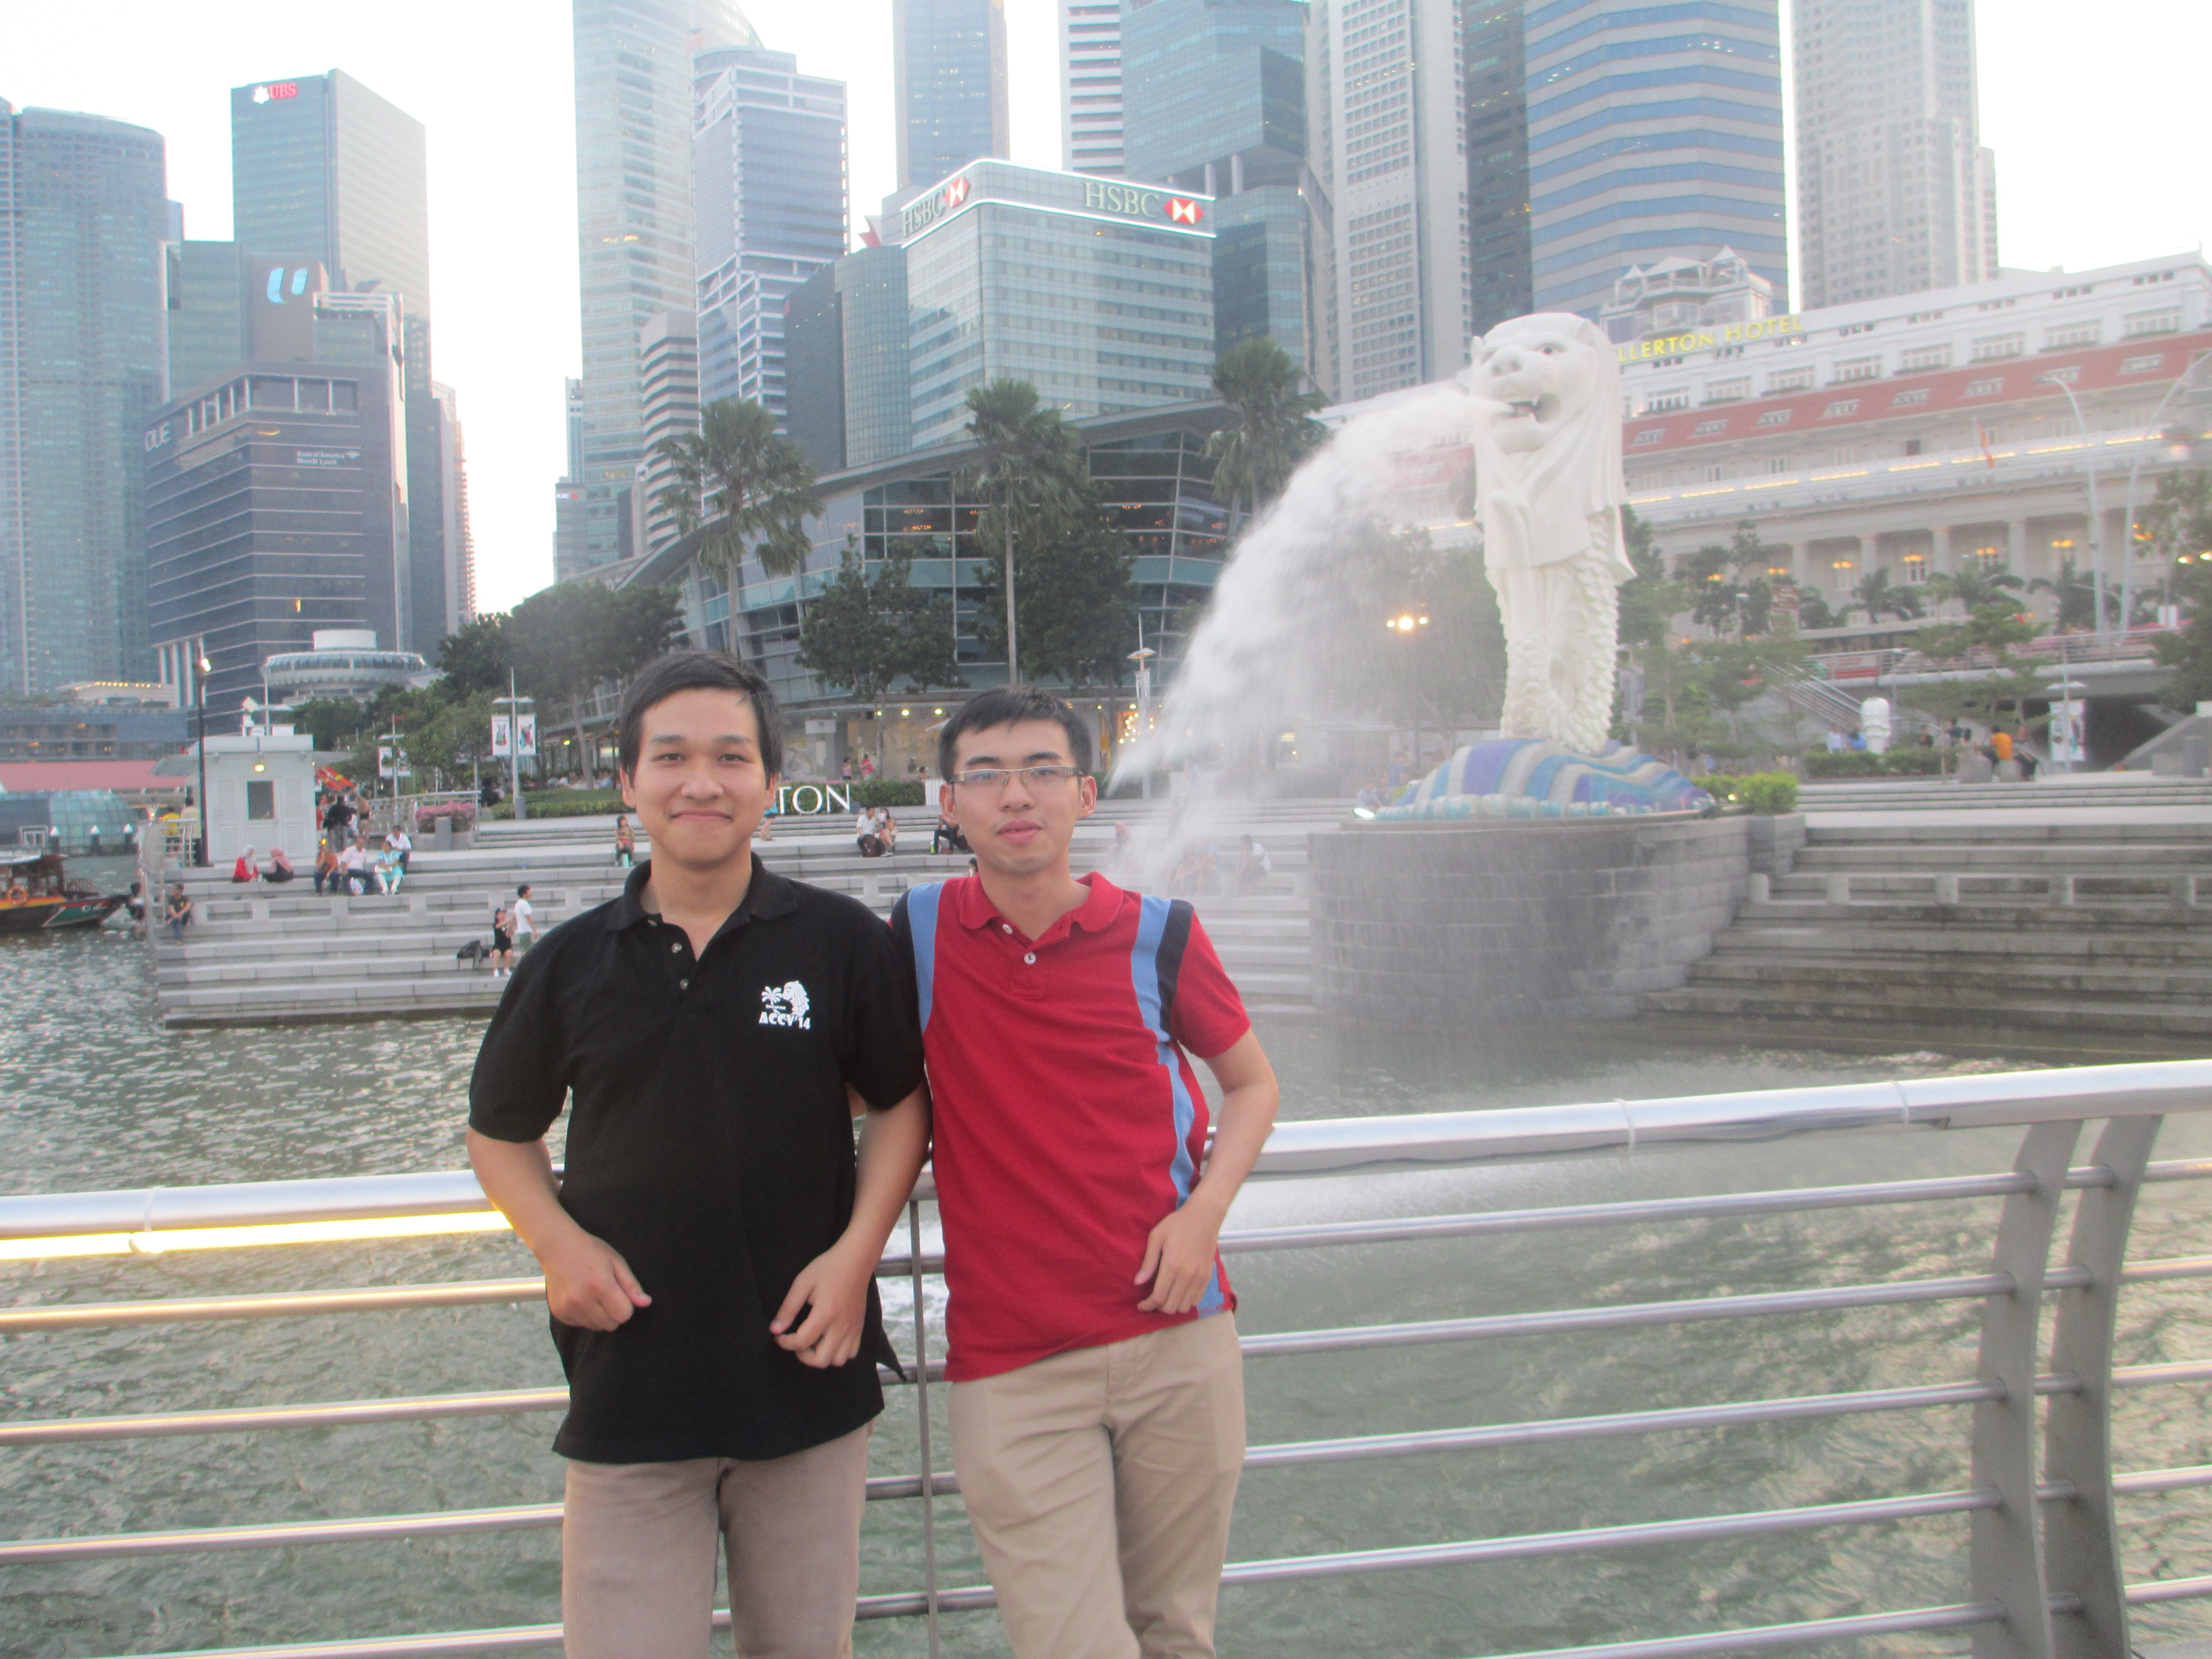
\includegraphics[width = 2in]{singapore_3.jpg}}
	\subfloat{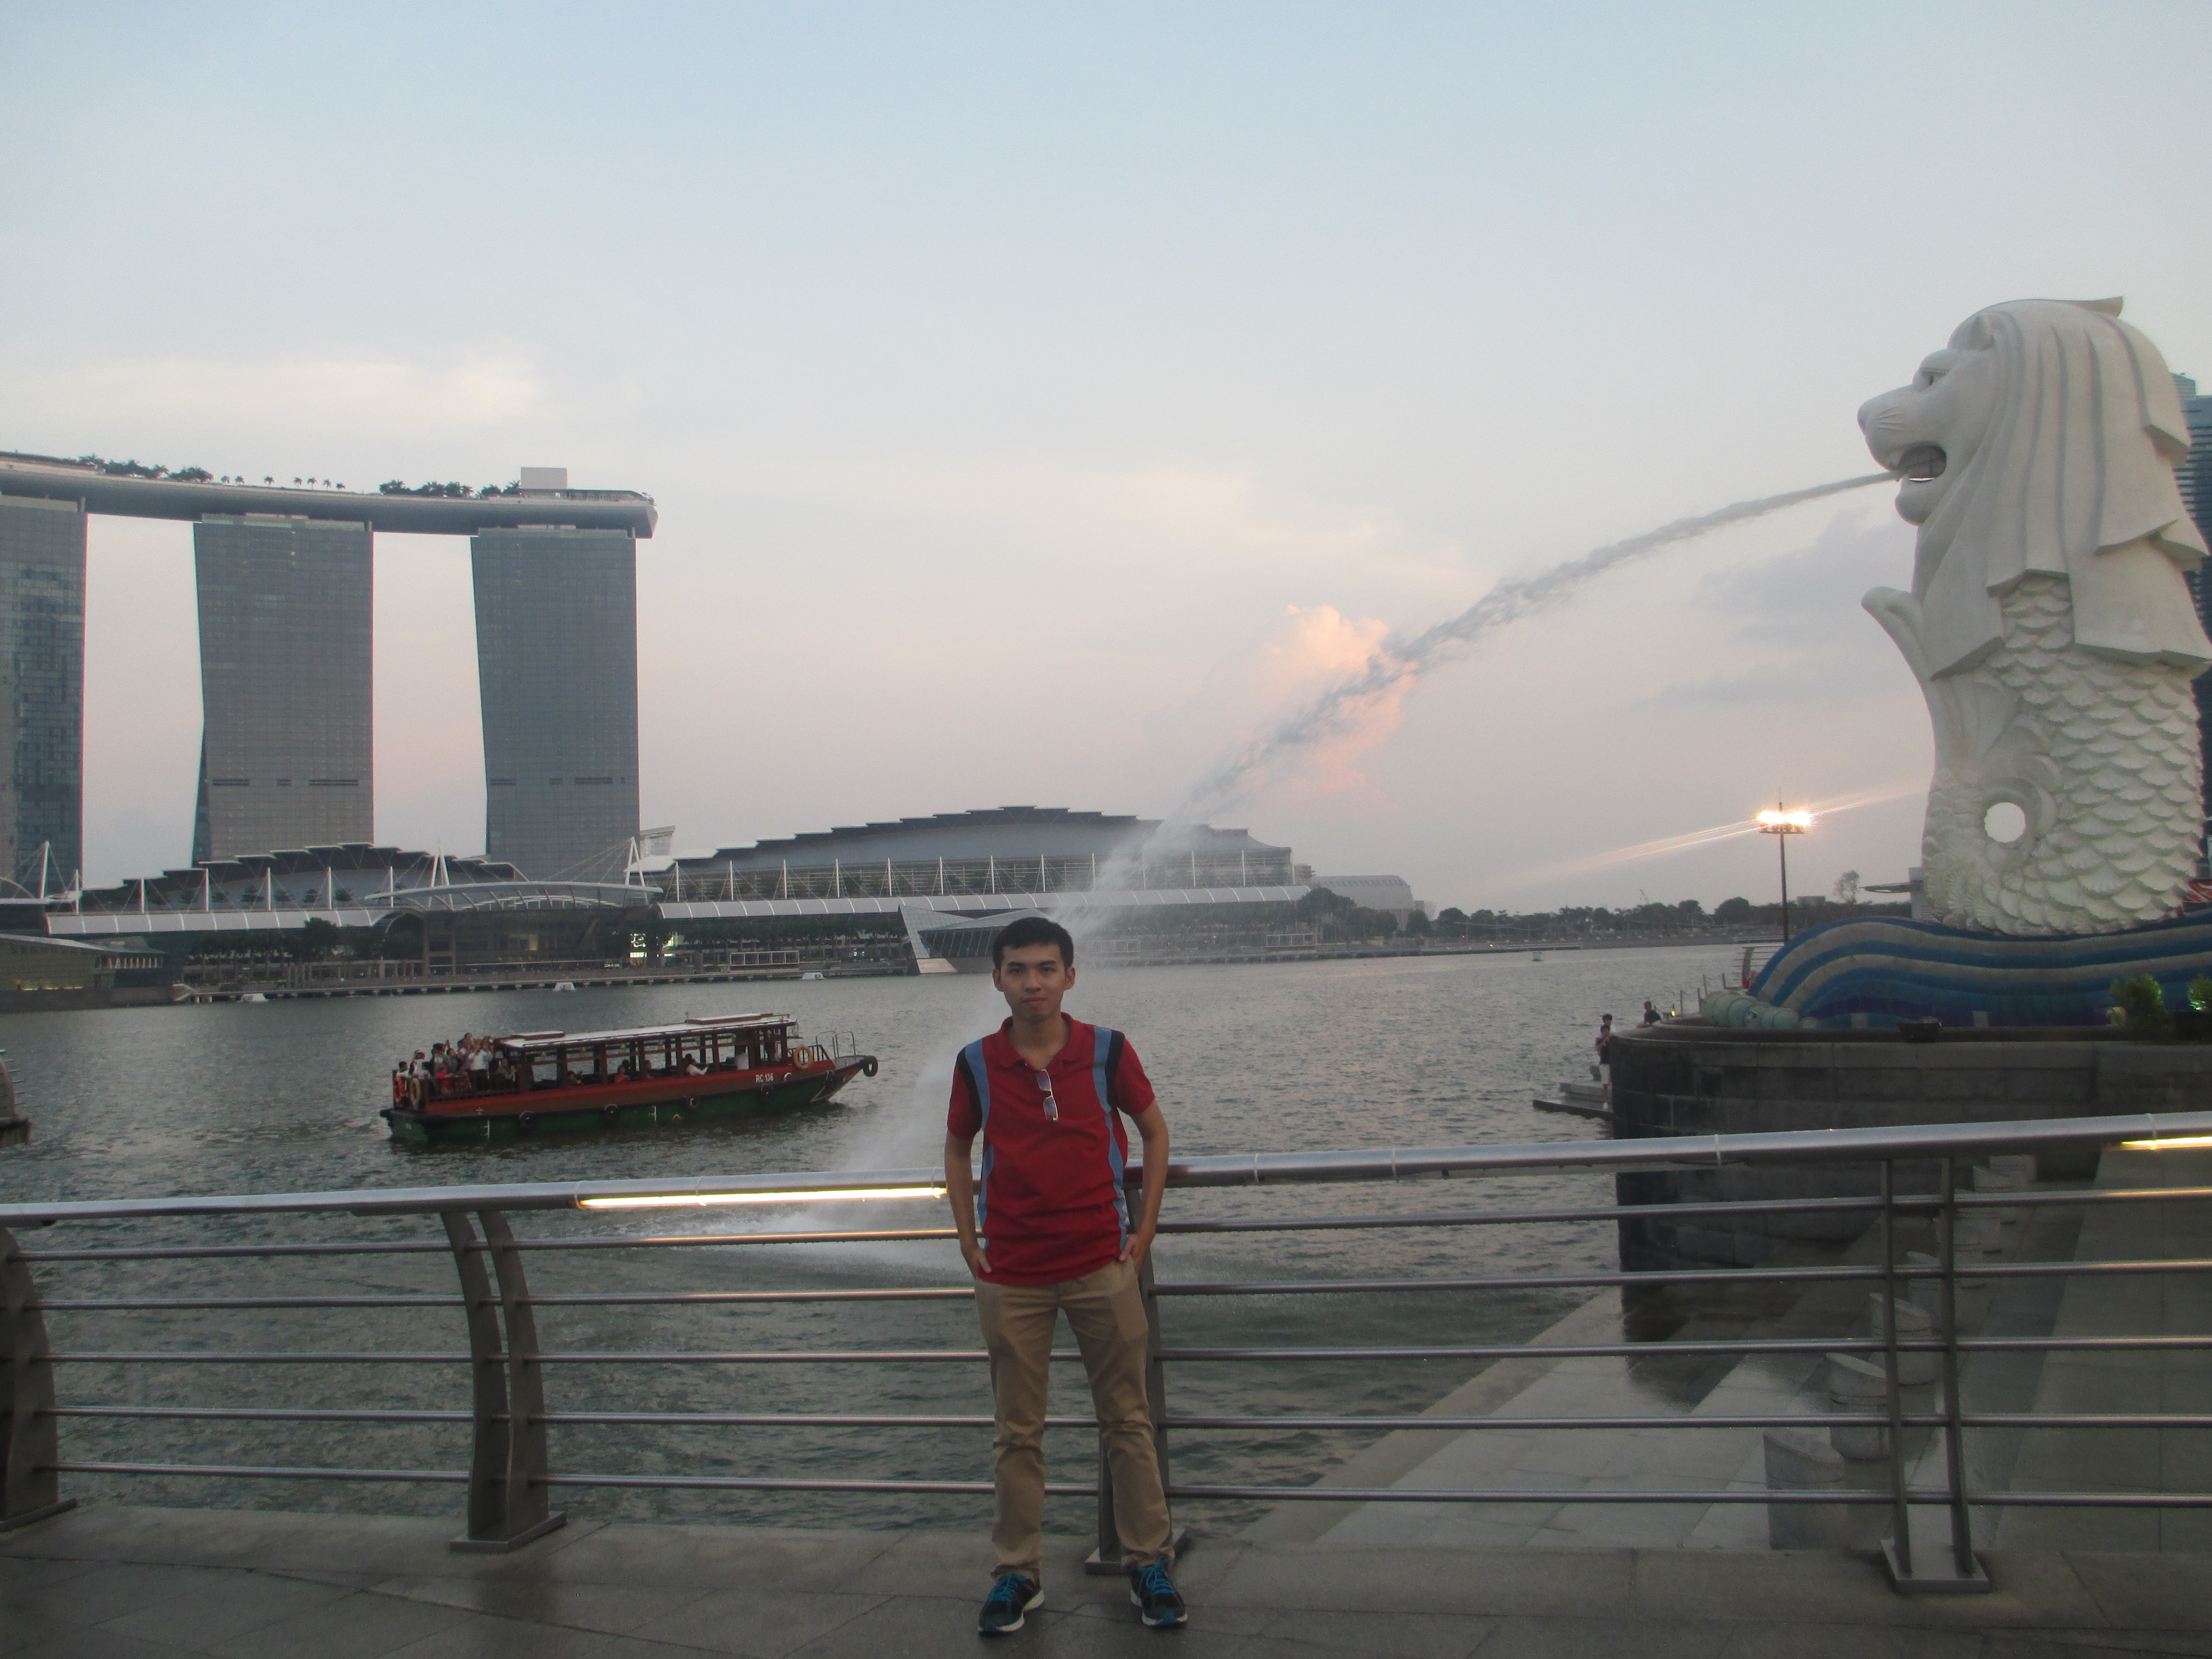
\includegraphics[width = 2in]{singapore_4.jpg}}
    \caption{Class 2, \#First\_time\_in\_Singapore}
    \label{fig:class_2}
\end{figure}

\begin{figure}
    \centering
	\subfloat{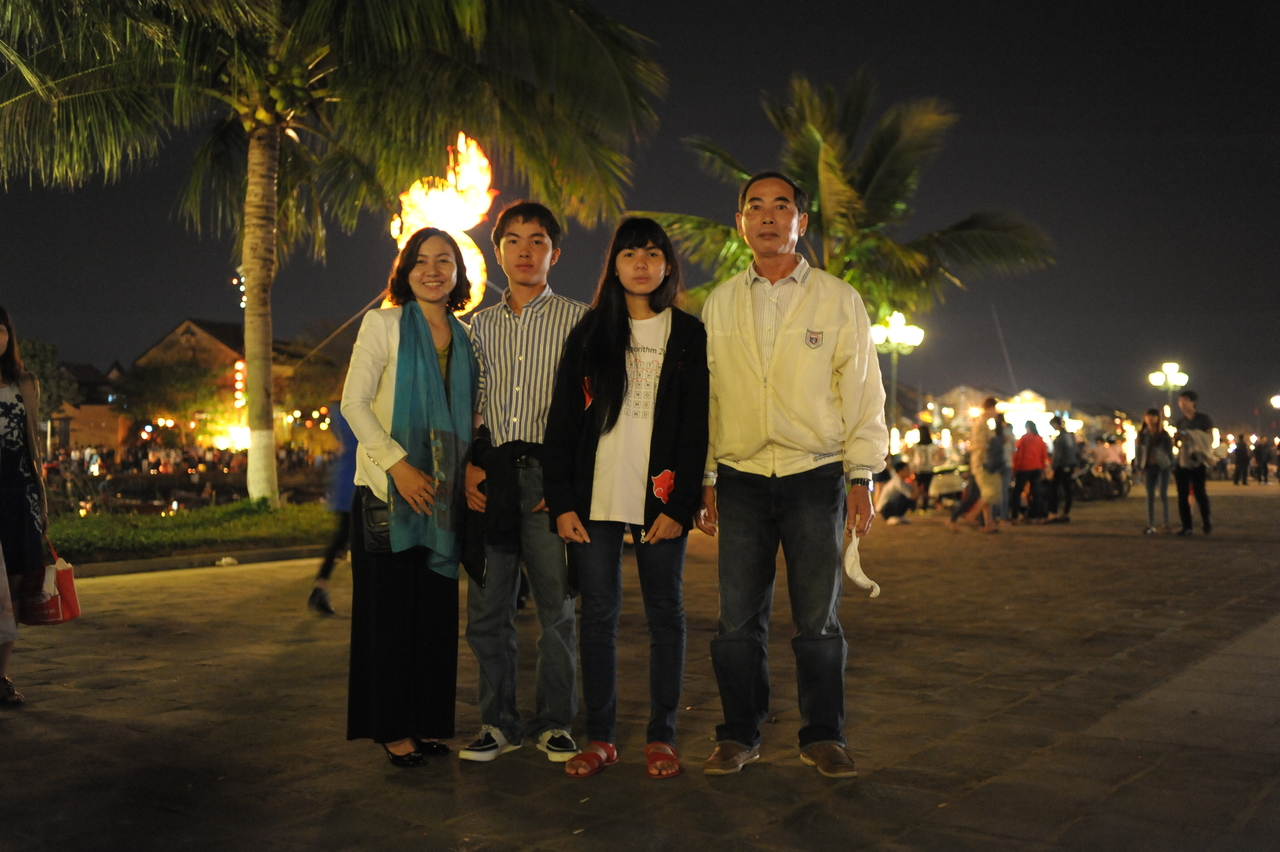
\includegraphics[width = 2in]{hoian_3.jpg}}
	\subfloat{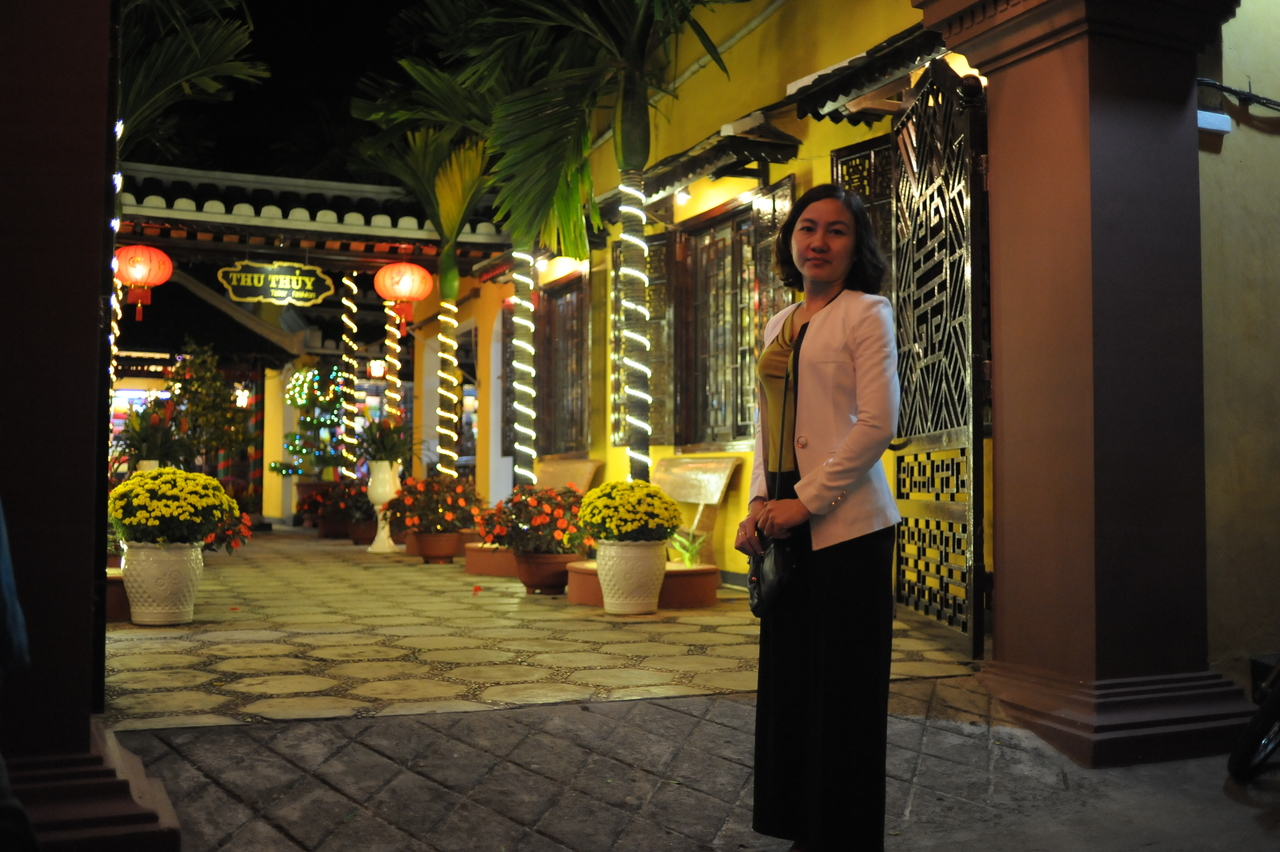
\includegraphics[width = 2in]{hoian_7.jpg}}
	\subfloat{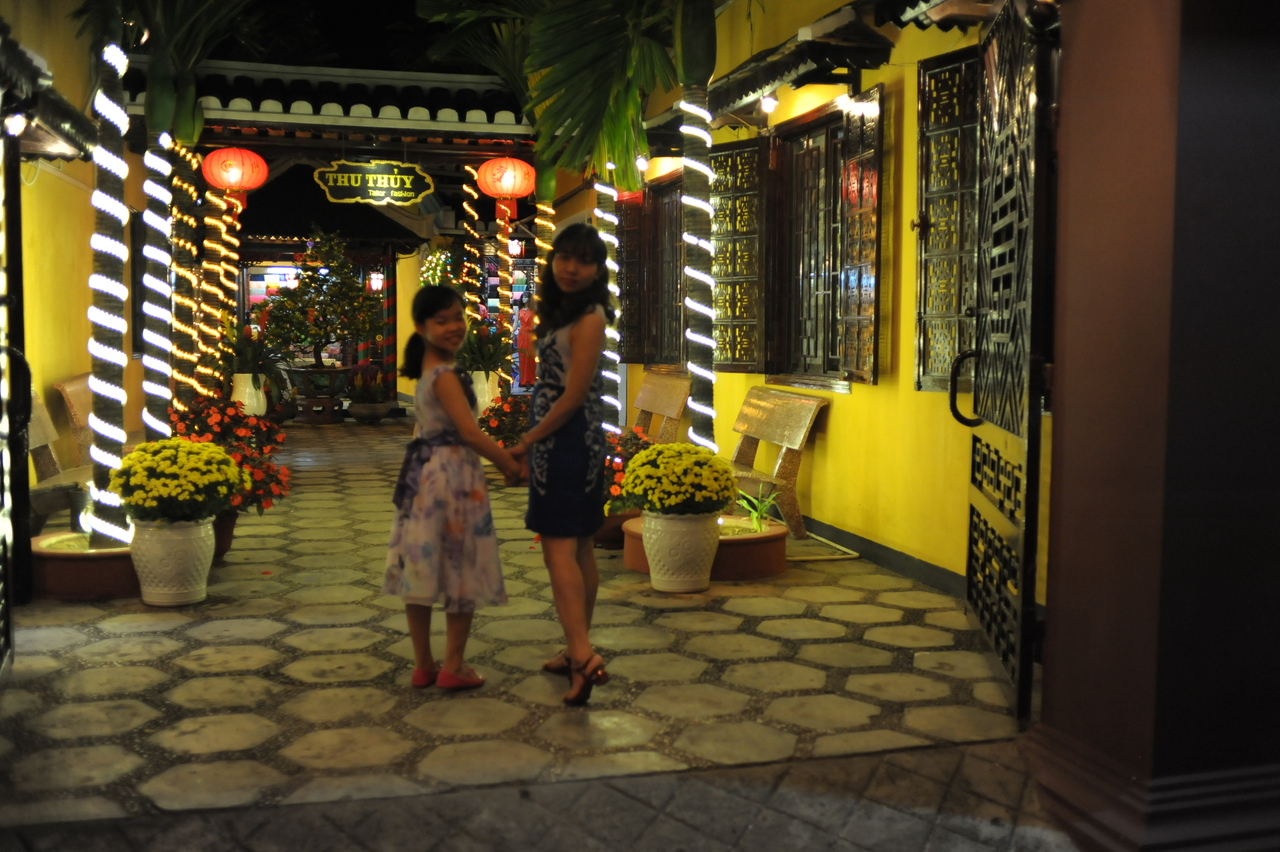
\includegraphics[width = 2in]{hoian_11.jpg}}
    \caption{Class 3, \#Hoi\_An\_with\_family}
    \label{fig:class_3}
\end{figure}

\begin{figure}
    \centering
	\subfloat{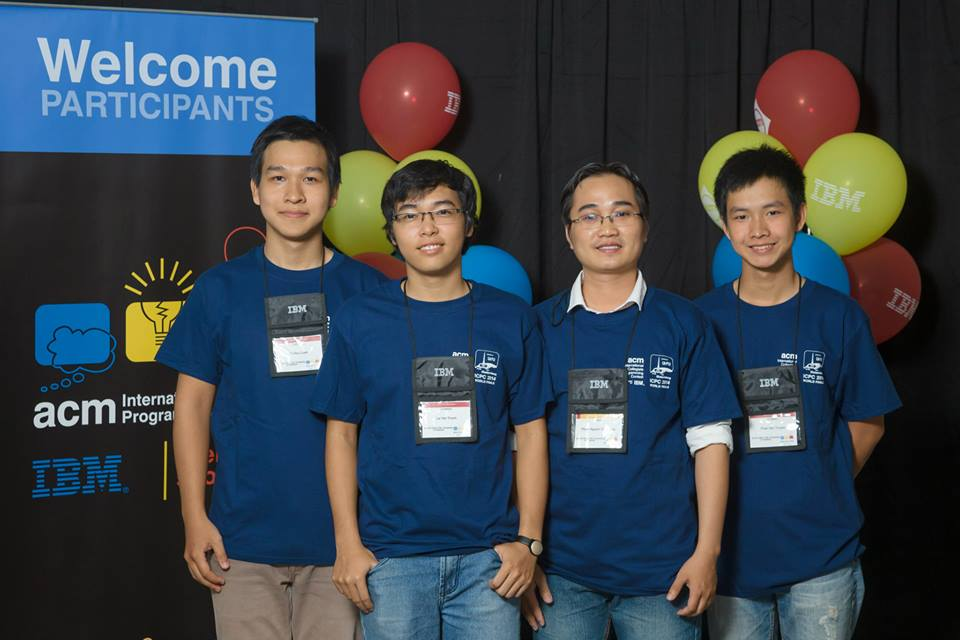
\includegraphics[width = 2in]{icpc_1.jpg}}
	\subfloat{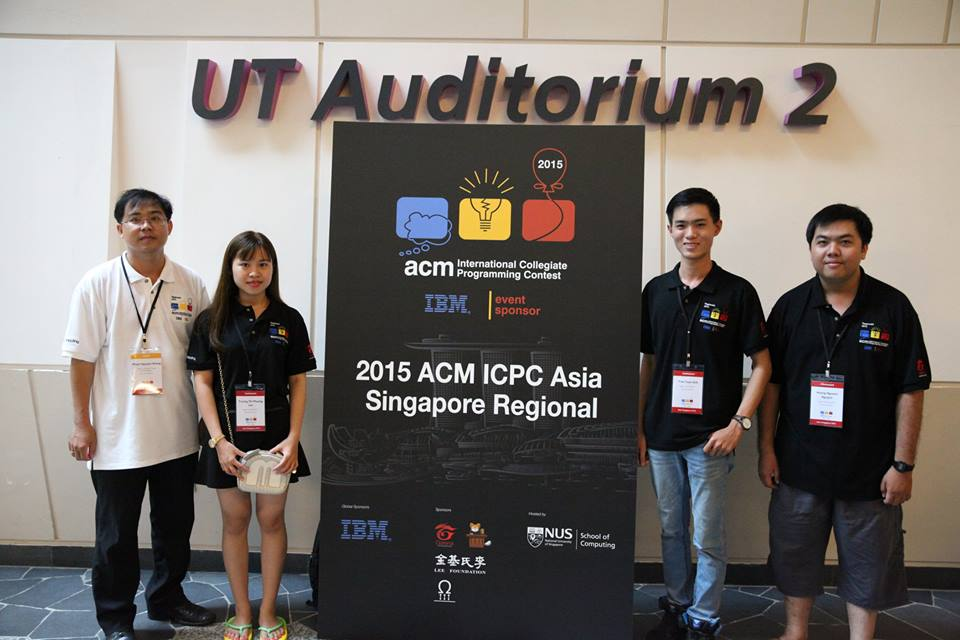
\includegraphics[width = 2in]{icpc_7.jpg}}
	\subfloat{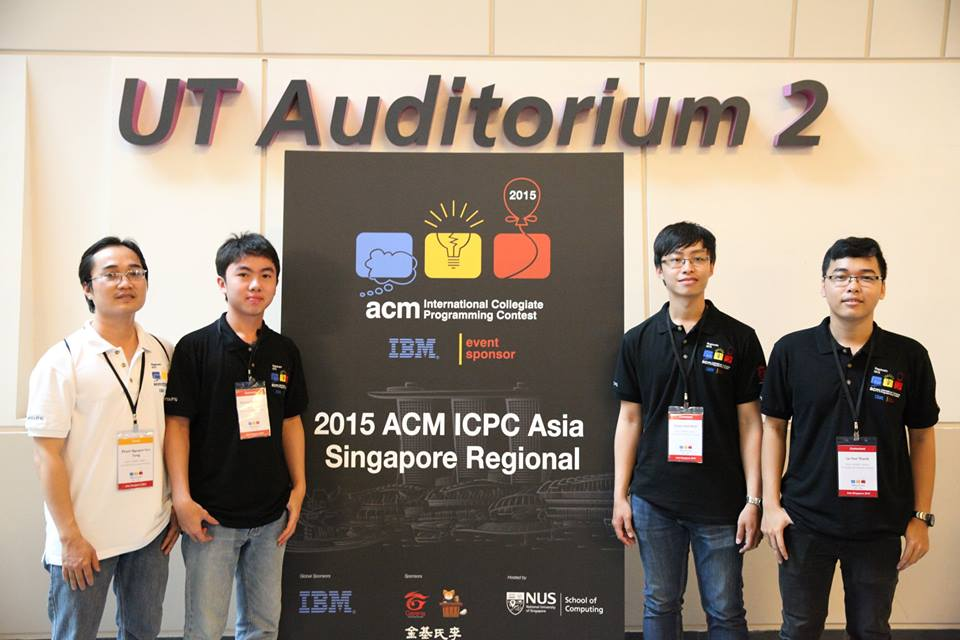
\includegraphics[width = 2in]{icpc_8.jpg}}
    \caption{Class 4, \#My\_favorite\_competition}
    \label{fig:class_4}
\end{figure}

\begin{figure}
    \centering
	\subfloat{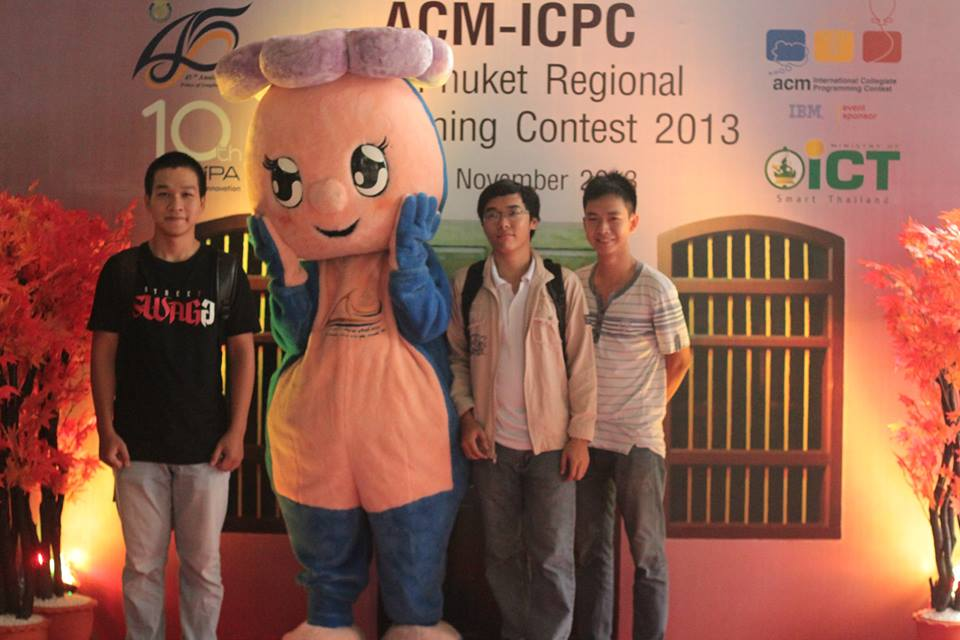
\includegraphics[width = 2in]{thailand_2.jpg}}
	\subfloat{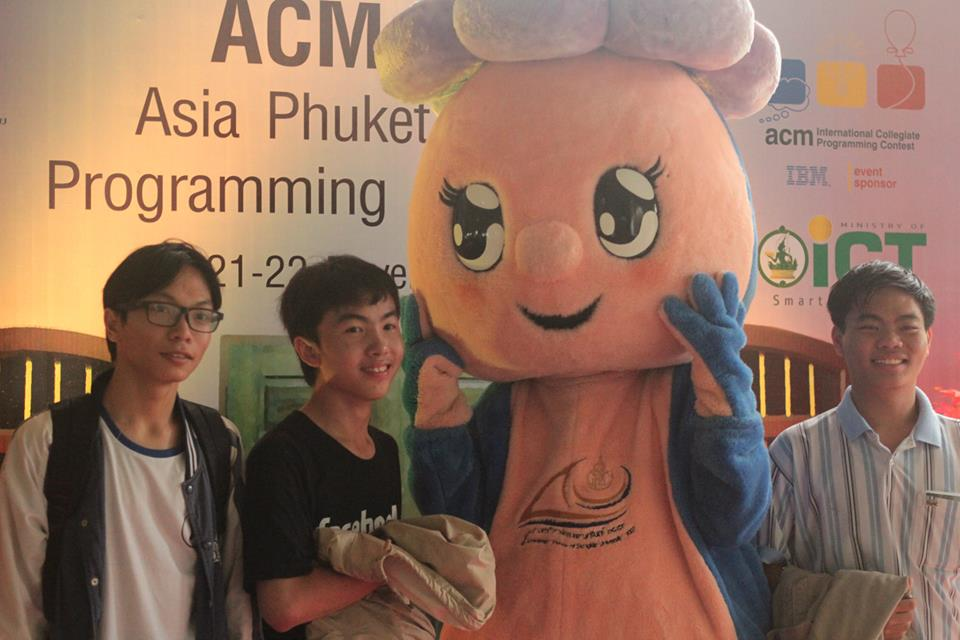
\includegraphics[width = 2in]{thailand_3.jpg}}
	\subfloat{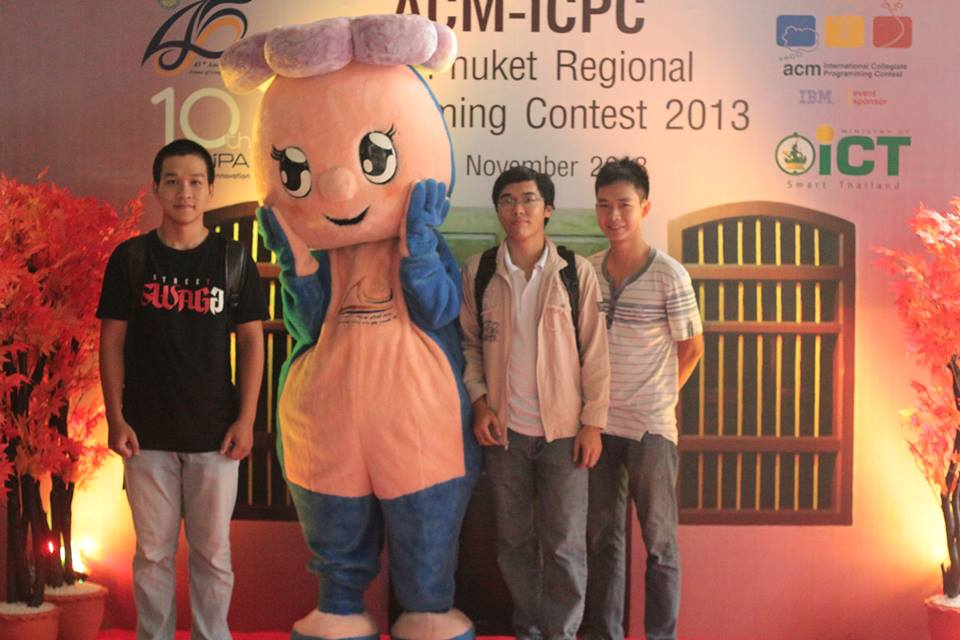
\includegraphics[width = 2in]{thailand_4.jpg}}
    \caption{Class 5, \#My\_first\_Regional}
    \label{fig:class_5}
\end{figure}

\begin{figure}
    \centering
	\subfloat{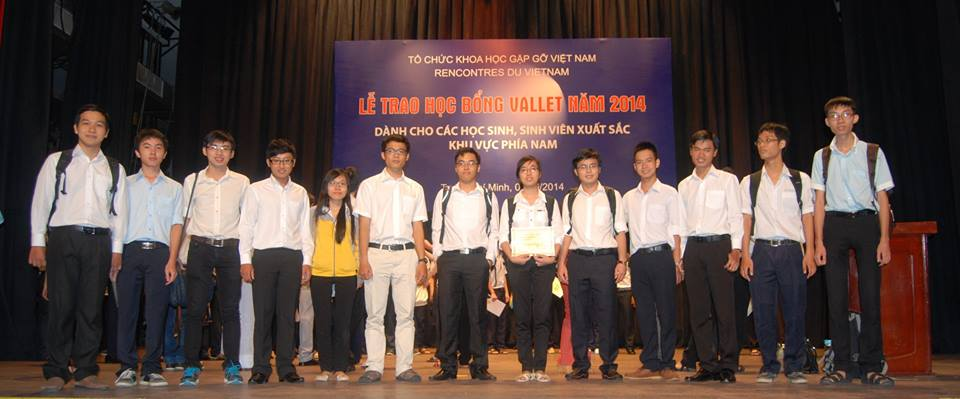
\includegraphics[width = 2in]{vallet_1.jpg}}
	\subfloat{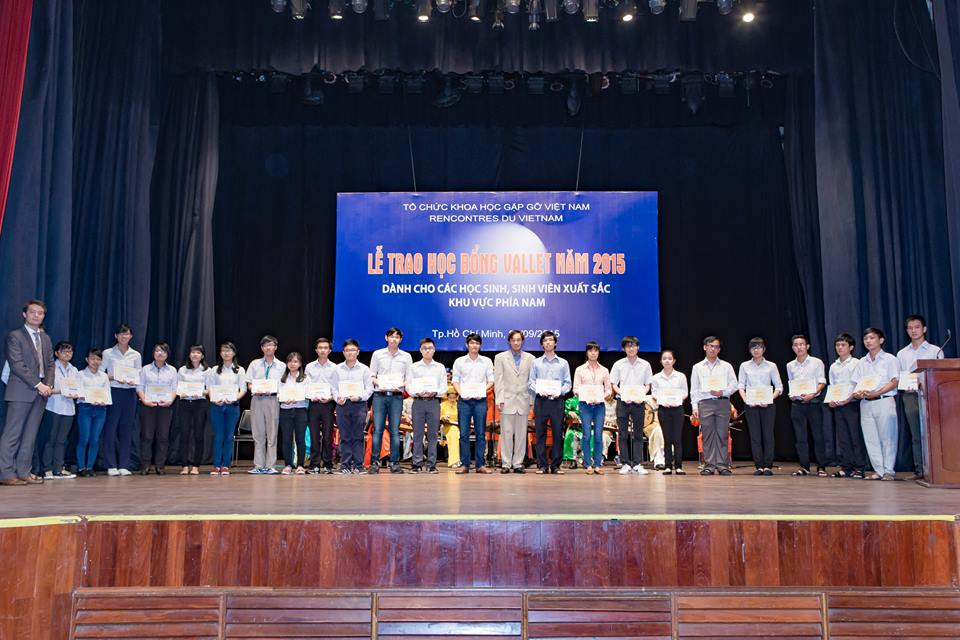
\includegraphics[width = 2in]{vallet_4.jpg}}
	\subfloat{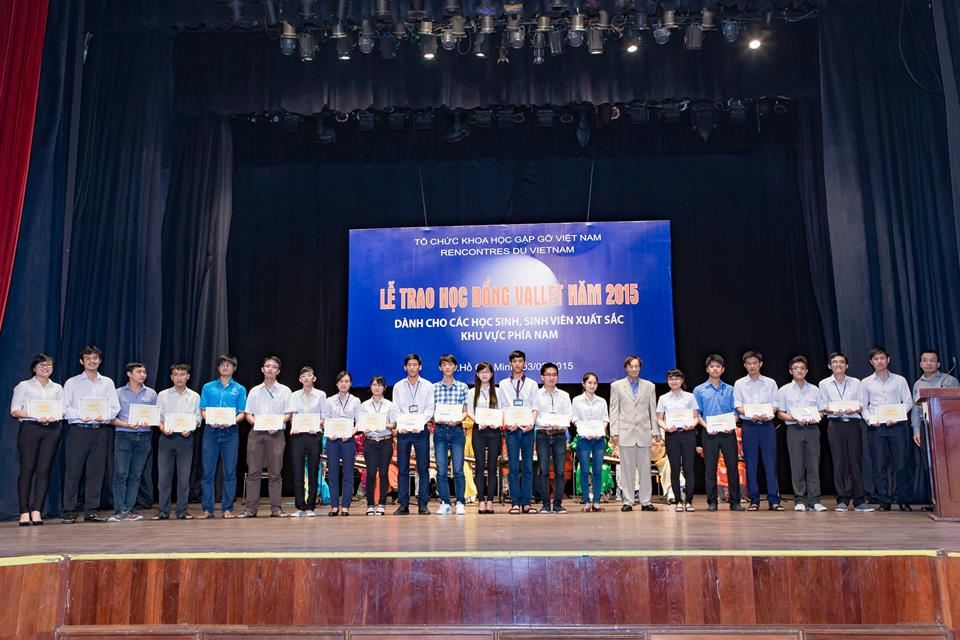
\includegraphics[width = 2in]{vallet_5.jpg}}
    \caption{Class 6, \#Odon\_Vallet\_scholarship}
    \label{fig:class_6}
\end{figure}